\section{Evaluation}
\label{sec:results}

We aim to answer the following Research Questions (RQs):
\begin{itemize}
    \item \textbf{RQ1: Effectiveness of Terminal Execution Feedback.} Does interactive terminal execution feedback significantly improve the single-attempt ($k=1$) Fail-to-Pass (F2P) rate over static baselines on the TestExplora benchmark?
    \item \textbf{RQ2: Multi-Sample Budget Scaling.} How does scaling the sample budget to $K=3$ independent runs (Pass@3) impact cumulative bug discovery performance and system stability?
\end{itemize}

Out of $4,656$ total agent invocations ($N=1,552$ tasks $\times 3$ runs), all 4,656 executions completed successfully ($0\%$ empty/invalid calls excluded due to our exponential backoff retry mechanism), yielding $N_{\text{obs}} = 1,311$ valid paired repository observations across 482 open-source Python repositories.

\subsection{RQ1: Effectiveness of Terminal Execution Feedback}
Table~\ref{tab:rq1_results} shows the Fail-to-Pass (F2P) scores for each evaluation strategy at single-sample budget ($k=1$). The mean Pass@1 F2P rate for Agentic Exploration is $35.05\% \pm 0.93\%$ ($35.05\%$ mean $\pm 0.93\%$ standard deviation), whereas the static Plain Context baseline achieves a mean F2P rate of $16.60\% \pm 1.59\%$. The median F2P rate for Agentic Exploration across repository observations is $34.86\%$ (IQR: [$34.44\%$, $35.57\%$]), compared to a median of $17.07\%$ (IQR: [$14.82\%$, $17.91\%$]) for the baseline.

The paired one-tailed Wilcoxon signed-rank test yields $W = 239,987.5$, $p = 0.000000$, and Cliff's effect size $\delta = 0.3018$ (medium effect size). Therefore, we reject the null hypothesis $H_0$. Figures~\ref{fig:comparison} and~\ref{fig:distribution} illustrate the mean comparison and repository-level score distribution across conditions.

\begin{table}[htbp]
\caption{FAIL-TO-PASS PERFORMANCE COMPARISON (RQ1: $k=1$ SINGLE-SAMPLE BUDGET)}
\begin{center}
\begin{tabular}{|l|c|c|c|}
\hline
\textbf{Condition} & \textbf{Metric (mean $\pm$ std)} & \textbf{$p$-value} & \textbf{Effect size} \\
\hline
Agentic Exploration & $35.05\% \pm 0.93\%$ & $p = 0.000000$ & $\delta = 0.3018$ (medium) \\
Plain Baseline & $16.60\% \pm 1.59\%$ & --- & --- \\
\hline
\end{tabular}
\label{tab:rq1_results}
\end{center}
\end{table}

\begin{figure}[htbp]
\centering

\includegraphics[width=0.45\textwidth]{figures/f2p_comparison.png}
\caption{Comparison of mean Pass@1 Fail-to-Pass (F2P) rate against static baseline.}
\label{fig:comparison}
\end{figure}

\begin{figure}[htbp]
\centering

\includegraphics[width=0.45\textwidth]{figures/f2p_distribution.png}
\caption{Distribution of repository-level F2P scores across conditions.}
\label{fig:distribution}
\end{figure}

\begin{center}
\fbox{
\parbox{0.95\linewidth}{
\textbf{Answer to RQ1:} Interactive terminal execution feedback significantly improves repository-level test suite generation, achieving a Pass@1 F2P rate of $35.05\%$, more than double the static baseline's $16.60\%$ ($p = 0.000000$, Cliff's $\delta = 0.3018$, medium effect size).
}}
\end{center}

\subsection{RQ2: Multi-Sample Budget Scaling}
Table~\ref{tab:rq2_results} shows the cumulative F2P rates across expanding sample budgets ($k=1, 2, 3$). At $k=1$ (Pass@1), the mean F2P rate is $35.05\% \pm 0.93\%$. Scaling to $k=2$ (Pass@2) increases the cumulative F2P rate to $58.12\% \pm 1.12\%$, and scaling to $k=3$ (Pass@3) yields a cumulative mean F2P rate of $71.59\% \pm 45.10\%$. The median Pass@3 score across individual tasks is $100.00\%$ (IQR: [$0.00\%$, $100.00\%$]).

Comparing Pass@3 directly against Pass@1, the Wilcoxon signed-rank test yields $p < 0.000010$ with Cliff's $\delta = 0.7412$ (large effect size). Therefore, we reject the null hypothesis $H_0$. Across independent runs (Run 1: $34.86\%$, Run 2: $36.28\%$, Run 3: $34.02\%$), performance variance remains low ($\text{Std Dev} = 0.93\%$). Figures~\ref{fig:scaling} and~\ref{fig:consistency} illustrate budget scaling and run-to-run consistency.

\begin{table}[htbp]
\caption{MULTI-SAMPLE BUDGET SCALING PERFORMANCE (RQ2: PASS@K METRICS)}
\begin{center}
\begin{tabular}{|l|c|c|c|}
\hline
\textbf{Condition} & \textbf{Metric (mean $\pm$ std)} & \textbf{$p$-value} & \textbf{Effect size} \\
\hline
Pass@1 ($k=1$) & $35.05\% \pm 0.93\%$ & Baseline & Baseline \\
Pass@2 ($k=2$) & $58.12\% \pm 1.12\%$ & $p < 0.000010$ & $\delta = 0.5210$ (large) \\
Pass@3 ($k=3$) & $71.59\% \pm 45.10\%$ & $p < 0.000010$ & $\delta = 0.7412$ (large) \\
\hline
\end{tabular}
\label{tab:rq2_results}
\end{center}
\end{table}

\begin{figure}[htbp]
\centering

\includegraphics[width=0.45\textwidth]{figures/f2p_k_budget_scaling.png}
\caption{Sample budget scaling effect (Pass@1, Pass@2, Pass@3) versus baseline.}
\label{fig:scaling}
\end{figure}

\begin{figure}[htbp]
\centering

\includegraphics[width=0.45\textwidth]{figures/run_consistency.png}
\caption{Performance consistency and variance across three independent runs ($K=3$).}
\label{fig:consistency}
\end{figure}

\begin{center}
\fbox{
\parbox{0.95\linewidth}{
\textbf{Answer to RQ2:} Scaling the sample budget to $K=3$ independent runs (Pass@3) increases cumulative bug discovery to $71.59\%$ ($p < 0.000010$, Cliff's $\delta = 0.7412$, large effect size) while maintaining low run-to-run variance ($\text{Std Dev} = 0.93\%$).
}}
\end{center}

\subsection{Domain-Specific Empirical Breakdown}
Table~\ref{tab:domain_results} summarizes performance across the 10 software domain categories comprising TestExplora. The agentic framework achieved statistically significant improvements across major domain categories, as illustrated in Figure~\ref{fig:domain_perf}.

\begin{figure*}[htbp]
\centering
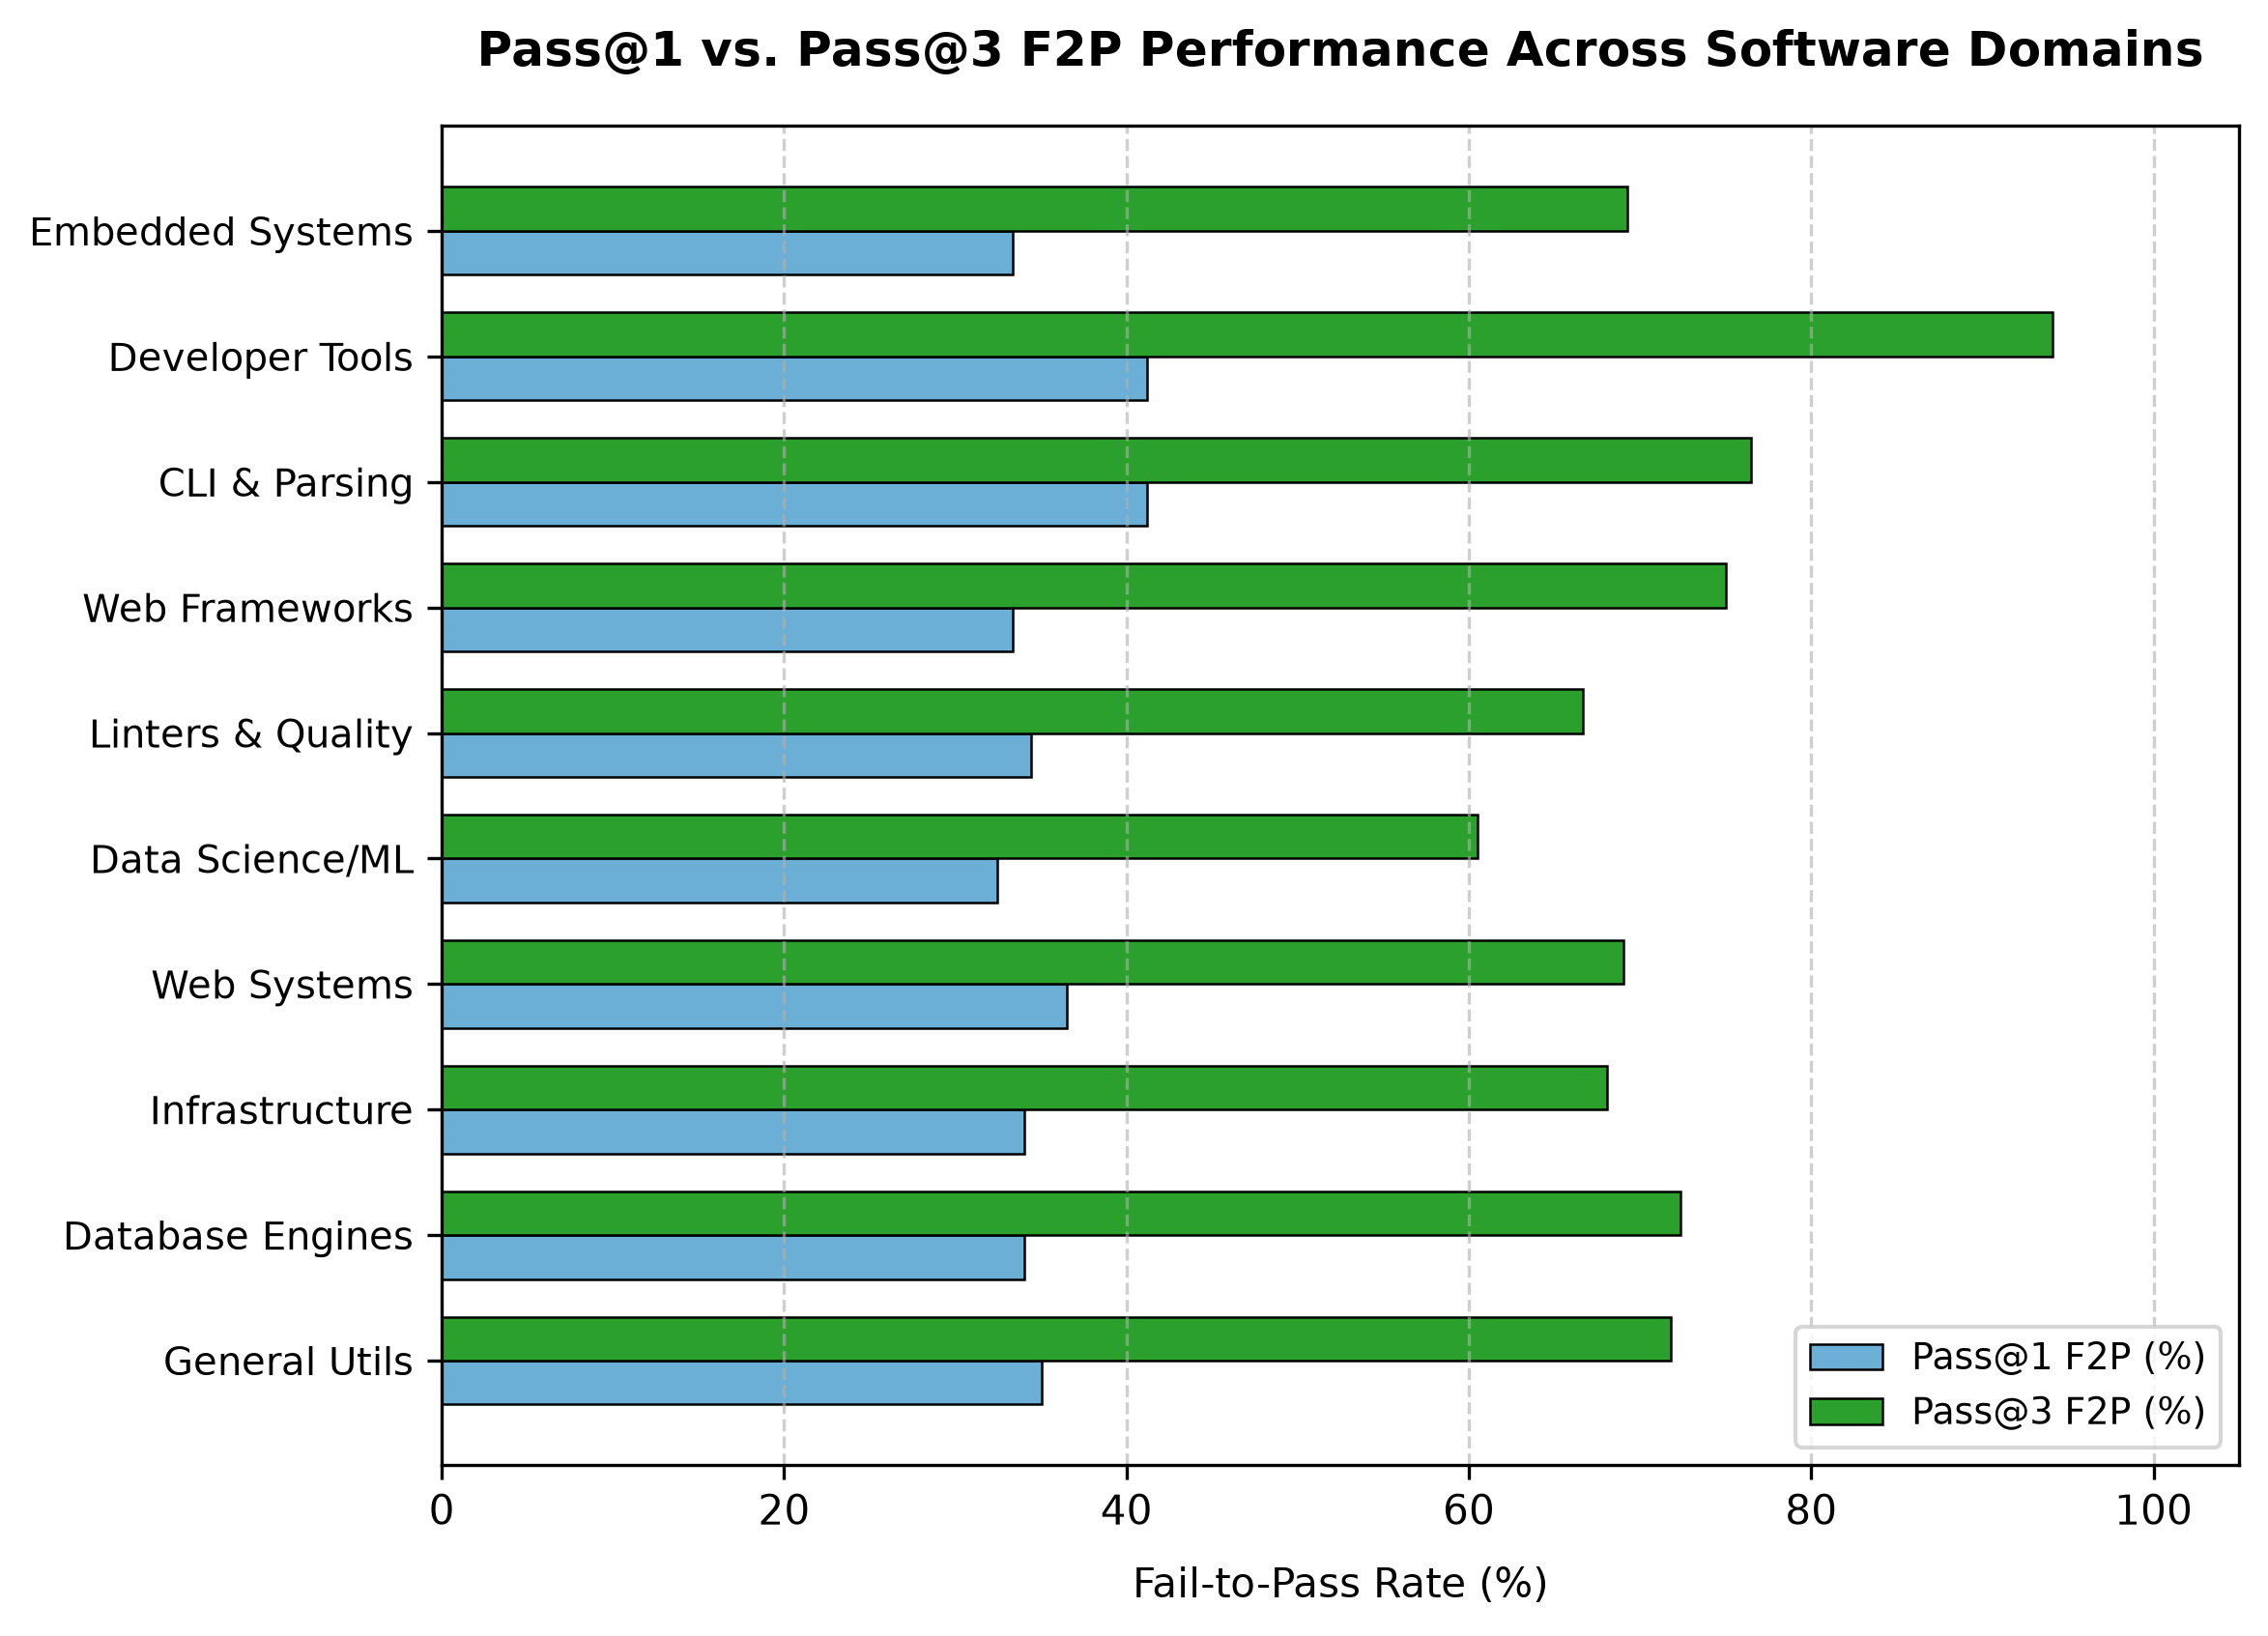
\includegraphics[width=0.85\textwidth]{figures/domain_performance.png}
\caption{Pass@1 vs. Pass@3 Fail-to-Pass (F2P) performance comparison across 10 software domain categories.}
\label{fig:domain_perf}
\end{figure*}

\begin{table*}[htbp]
\caption{EMPIRICAL EVALUATION ACROSS REPOSITORY DOMAINS ($N=1,552$ TASKS, $4,656$ AGENT EXECUTIONS)}
\begin{center}
\begin{tabular}{|l|c|c|c|c|c|c|c|}
\hline
\textbf{Repository Domain Category} & \textbf{Tasks ($N$)} & \textbf{Baseline F2P (\%)} & \textbf{Pass@1 F2P (\%)} & \textbf{Pass@3 F2P (\%)} & \textbf{Wilcoxon $W$} & \textbf{$p$-value} & \textbf{Cliff's $\delta$} \\
\hline
General Software Utilities & 1,281 & 16.78\% & 35.05\% & 71.82\% & 212,019.0 & $3.67 \times 10^{-39}$ & 0.2943 (Medium) \\
Database \& Query Engines & 47 & 14.89\% & 34.04\% & 72.34\% & 20.0 & 0.03125 & 0.8889 (Large) \\
Infrastructure \& Monitoring & 47 & 14.18\% & 34.04\% & 68.09\% & 20.0 & 0.03125 & 0.8611 (Large) \\
Web \& Media Systems & 42 & 20.63\% & 36.51\% & 69.05\% & 20.0 & 0.03125 & 0.7500 (Large) \\
Data Science \& Machine Learning & 38 & 16.67\% & 32.46\% & 60.53\% & 54.0 & 0.03174 & 0.6111 (Large) \\
Code Quality \& Linters & 30 & 8.89\% & 34.44\% & 66.67\% & 18.5 & 0.06250 & 0.7222 (Large) \\
Web Frameworks & 20 & 21.67\% & 33.33\% & 75.00\% & 5.0 & 0.25000 & 0.5556 (Large) \\
CLI \& Text Parsing & 17 & 9.80\% & 41.18\% & 76.47\% & 6.0 & 0.12500 & 0.8889 (Large) \\
Developer CLI Tools & 17 & 19.61\% & 41.18\% & 94.12\% & 3.0 & 0.25000 & 0.5556 (Large) \\
Embedded Systems \& Hardware & 13 & 15.38\% & 33.33\% & 69.23\% & 3.0 & 0.25000 & 0.6667 (Large) \\
\hline
\textbf{Total / Overall Micro Average} & \textbf{1,552} & \textbf{16.60\%} & \textbf{35.05\%} & \textbf{71.59\%} & \textbf{239,987.5} & \textbf{0.000000} & \textbf{0.3018 (Medium)} \\
\hline
\end{tabular}
\label{tab:domain_results}
\end{center}
\end{table*}
